\section{CI/CD}
\label{CICD}

CI e CD sono due acronimi particolarmente usati nelle pratiche di sviluppo software moderno. Esse collaborano tra di loro per il raggiungimento di uno sviluppo software rapido ed efficace. 

\begin{figure}[H]
\centering
	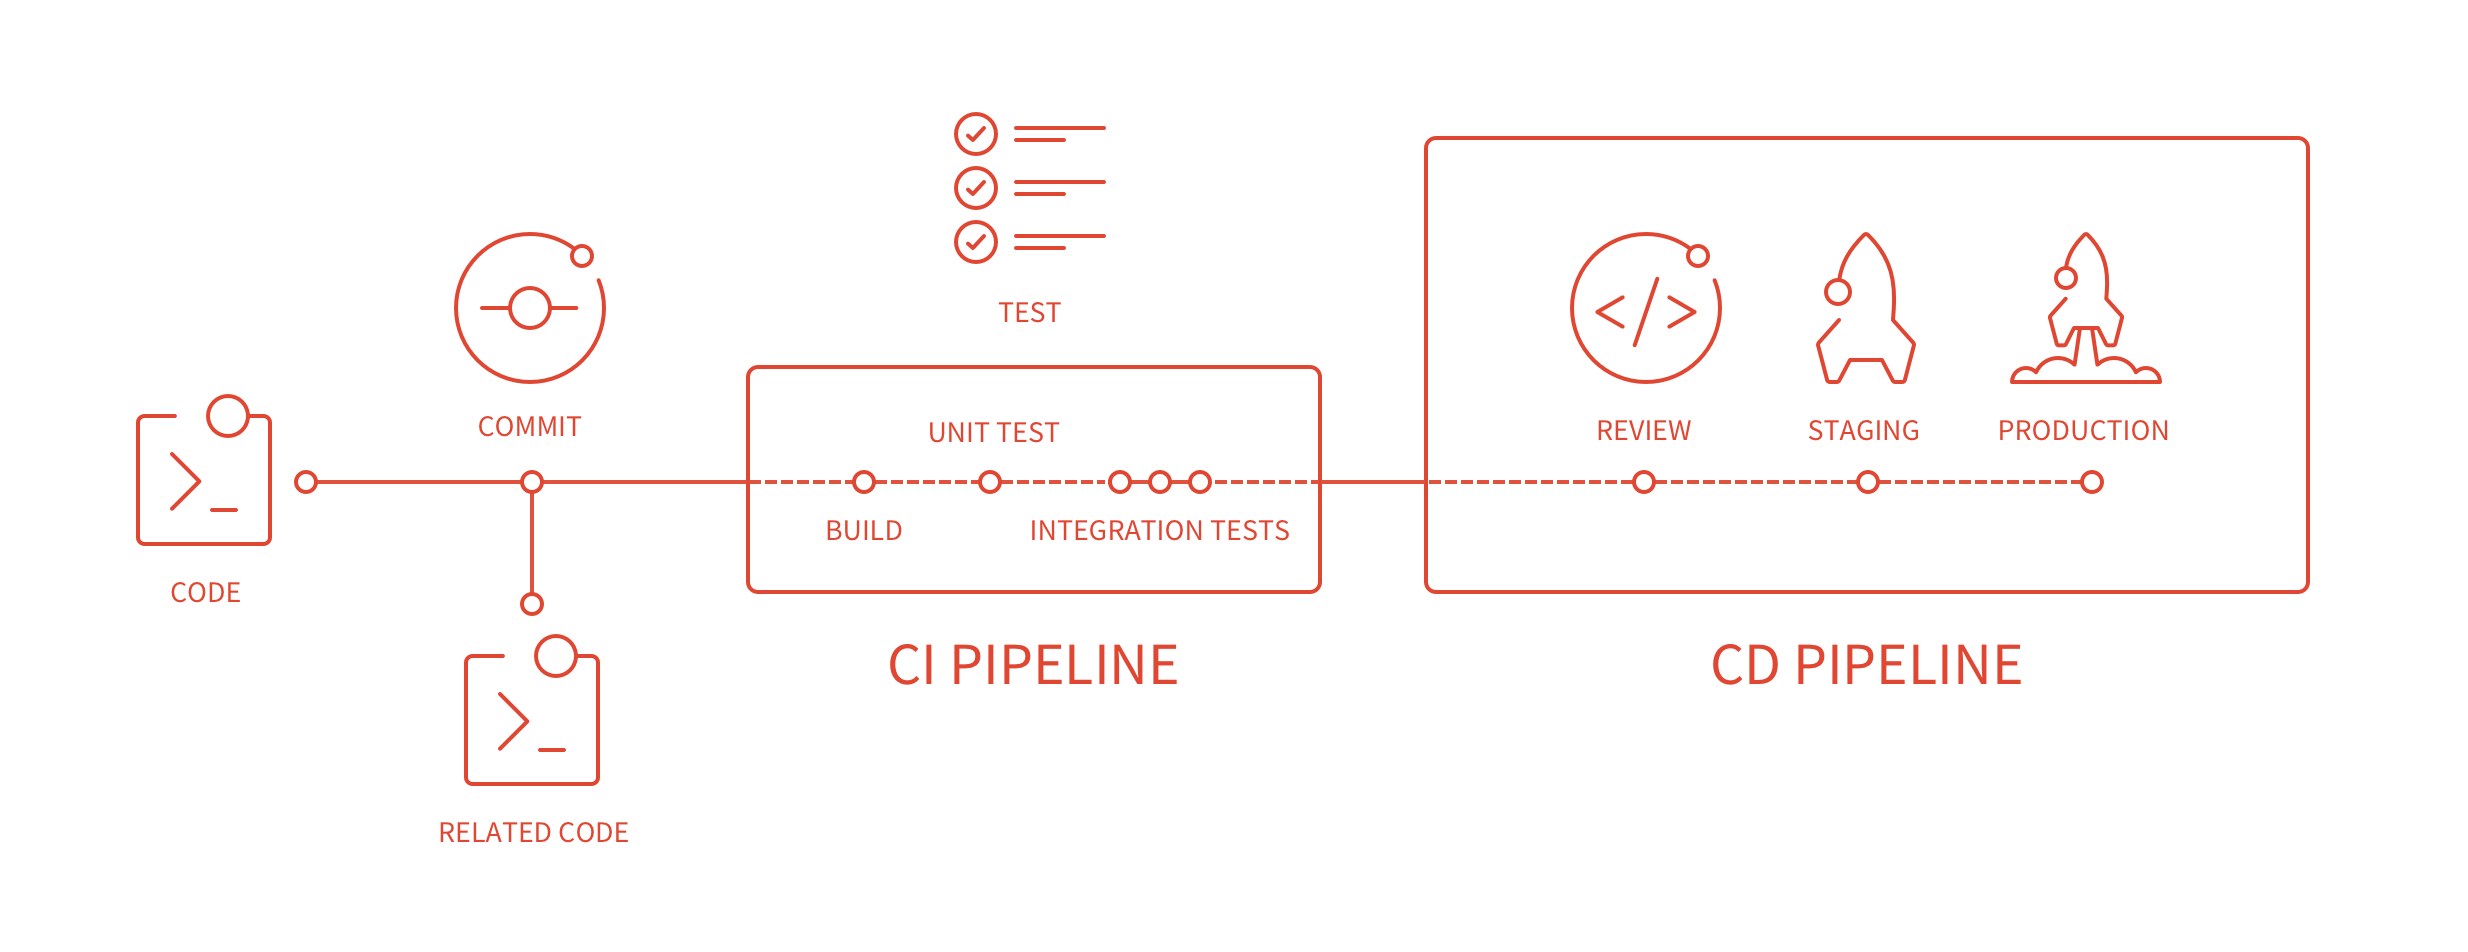
\includegraphics[width=0.9\linewidth]{./images/cicd_pipeline_gitlab.png} 
	\caption{Rappresentazione del processo di CI/CD \url{ https:// docs.gitlab.com/ee/ci/}}
	\label{vmodel}
\end{figure}

\subsection{CI}

La CI (Continuous integration) è una filosofia di sviluppo e set di pratiche con l'obbiettivo di guidare un team di sviluppo a implementare cambiamenti e testing frequenti sul repository del codice. 
L'obbiettivo della CI è di stabilire un modo coerente e automatico per costruire e testare applicazioni. Con la coerenza del processo di integrazione, i team hanno  maggiori probabilità di modificare il codice più frequentemente, il che porta a una migliore collaborazione e qualità del software, riducendone i tempi. \\
Per implementare questa filosofia ci sono dei costi: 
\begin{itemize}
	\item Il team di sviluppo dovrà scrivere test automatici per ogni nuova feature, miglioramento o bug fix;
	\item Viene impostato un server dedicato, il quale monitora il repository principale e testa il codice con i test precedentemente scritti;
	\item Gli sviluppatori devono mergiare le modifiche effettuate con quelle degli altri sviluppatori il più frequentemente possibile, almeno una volta al giorno. 
\end{itemize}

Dai precedenti costi si ottiene: 
\begin{itemize}
	\item Vengono spediti meno bug in produzione poiché le regressioni vengono acquisite in anticipo dai test automatici;
	\item Costruire la versione è facile poiché tutti i problemi di integrazione sono stati risolti in anticipo; 
	\item Meno cambi di contesto, poiché gli sviluppatori sono allertati non appena la build si interrompe, dando la possibilità di sistemare prima di procedere con la successiva task;
	\item I costi dei test sono ridotti drasticamente. Il server dedicato può eseguire centinaia di test in pochi secondi; 
	\item Il team spende meno tempo a testare il prodotto e si concentra di più a migliorare la qualità.
\end{itemize}


\subsection{CD}
La CD (Continuous delivery) è un'estensione della continuous integration per poter assicurare di poter rilasciare rapidamente nuove modifiche ai clienti in modo sostenibile. Ciò significa che oltre ad aver automatizzato i test, si ha anche automatizzato il processo di rilascio e si può distribuire l'applicazione in qualsiasi momento. 
Affinché sia veramente efficace, è necessario distribuire la produzione il prima possibile per assicurarsi di rilasciare piccolo batch che siano facili da risolvere in caso di problemi. \\
Per implementare efficacemente la CD bisogna seguire i seguenti punti: 
\begin{itemize}
	\item Serve una solida base nella continuous integration e la suite di test deve coprire una certa percentuale della codebase; 
	\item Il rilascio deve essere automatizzato. Il trigger può essere manuale, ma una volta avviata la distribuzione non dovrebbe essere necessario l'intervento umano; 
	\item Il team dovrà adottare le flag di funzionalità in modo che le funzionalità incomplete non influiscano sui clienti durante la produzione. 
\end{itemize}

Dalle precedenti si ottiene: 
\begin{itemize}
\item La complessità della distribuzione del software è portata via. Il team non deve più prepararsi per il rilascio; 
\item Si può rilasciare molto più frequentemente, accelerando cosi il ciclo di feedback con i clienti; 
\item C'è meno pressione sulle decisioni per piccoli cambiamenti, incoraggiando dunque la iterazione più velocemente. 
\end{itemize}



% La \textbf{CI/CD} (Continuous integration / Continuous delivery) sono due filosofie applicate allo sviluppo moderno di software
